\section{Úvod}\label{sec:uvod}

Konečné (stavové) automaty představují abstraktní stroje reprezentující určitý výpočet nebo algoritmus. Z reálného světa můžeme za stavový automat považovat např. obyčejný vypínač, viz obrázek \ref{fig:vypinac}.
\begin{figure}[h]
    \begin{center}
        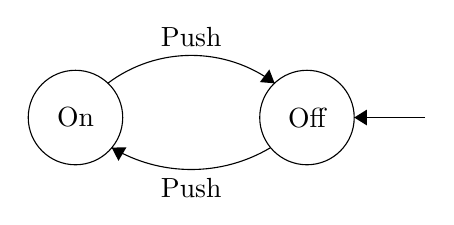
\begin{tikzpicture}[scale=0.2]
        \tikzstyle{every node}+=[inner sep=0pt]
        \draw [black] (29,-28.9) circle (3);
        \draw (29,-28.9) node {On};
        \draw [black] (43.7,-28.9) circle (3);
        \draw (43.7,-28.9) node {Off};
        \draw [black] (31.047,-26.727) arc (126.9692:53.0308:8.818);
        \fill [black] (41.65,-26.73) -- (41.31,-25.85) -- (40.71,-26.65);
        \draw (36.35,-24.45) node [above] {Push};
        \draw [black] (41.399,-30.806) arc (-59.10767:-120.89233:9.833);
        \fill [black] (31.3,-30.81) -- (31.73,-31.65) -- (32.24,-30.79);
        \draw (36.35,-32.7) node [below] {Push};
        \draw [black] (51.2,-28.9) -- (46.7,-28.9);
        \fill [black] (46.7,-28.9) -- (47.5,-29.4) -- (47.5,-28.4);
        \end{tikzpicture}
    \end{center}
    \caption{Schéma automatu pro vypínač.}
    \label{fig:vypinac}
\end{figure}
Příkladem praktického použití návrhu automatů je tzv. \emph{lexikální analýza}, kterou se budeme zabývat v kapitole~\smartref[][ v sekci \dots]{true}{chap:kompilatory}{o kompilátorech}. Na obrázku \ref{fig:automat-then} je vidět příklad konečného automatu rozpoznávající slovo \textit{then}.
\begin{figure}[h]
    \begin{center}
        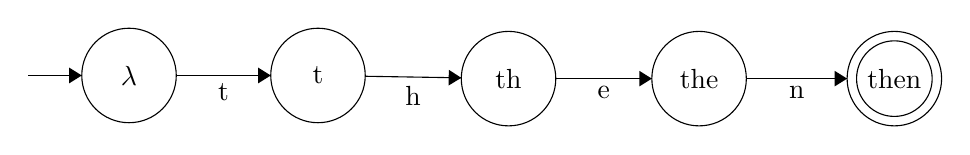
\begin{tikzpicture}[scale=0.2]
        \tikzstyle{every node}+=[inner sep=0pt]
        \draw [black] (17.7,-28.6) circle (3);
        \draw (17.7,-28.6) node {$\lambda$};
        \draw [black] (29.7,-28.6) circle (3);
        \draw (29.7,-28.6) node {t};
        \draw [black] (41.8,-28.8) circle (3);
        \draw (41.8,-28.8) node {th};
        \draw [black] (53.9,-28.8) circle (3);
        \draw (53.9,-28.8) node {the};
        \draw [black] (66.3,-28.8) circle (3);
        \draw (66.3,-28.8) node {then};
        \draw [black] (66.3,-28.8) circle (2.4);
        \draw [black] (11.3,-28.6) -- (14.7,-28.6);
        \fill [black] (14.7,-28.6) -- (13.9,-28.1) -- (13.9,-29.1);
        \draw [black] (20.7,-28.6) -- (26.7,-28.6);
        \fill [black] (26.7,-28.6) -- (25.9,-28.1) -- (25.9,-29.1);
        \draw (23.7,-29.1) node [below] {t};
        \draw [black] (32.7,-28.65) -- (38.8,-28.75);
        \fill [black] (38.8,-28.75) -- (38.01,-28.24) -- (37.99,-29.24);
        \draw (35.74,-29.22) node [below] {h};
        \draw [black] (44.8,-28.8) -- (50.9,-28.8);
        \fill [black] (50.9,-28.8) -- (50.1,-28.3) -- (50.1,-29.3);
        \draw (47.85,-29.3) node [below] {e};
        \draw [black] (56.9,-28.8) -- (63.3,-28.8);
        \fill [black] (63.3,-28.8) -- (62.5,-28.3) -- (62.5,-29.3);
        \draw (60.1,-29.3) node [below] {n};
        \end{tikzpicture}
        \end{center}
    \caption{Schéma automatu rozpoznávající slovo \texttt{then}.}
    \label{fig:automat-then}
\end{figure}

Jak tedy vlastně konečné automaty fungují? Vstup je reprezentován určitou \textbf{konečnou posloupností znaků}, tedy nějakým řetězcem neboli tzv. \textbf{slovem}, které daný automat zpracováva postupně po jednotlivých znacích. Na konci výpočtu vydá automat odpověď, zda vstup \textbf{přijal}, či \textbf{nepřijal} (viz obrázek \ref{fig:konecny-automat}).
\begin{figure}[h]
    \centering
    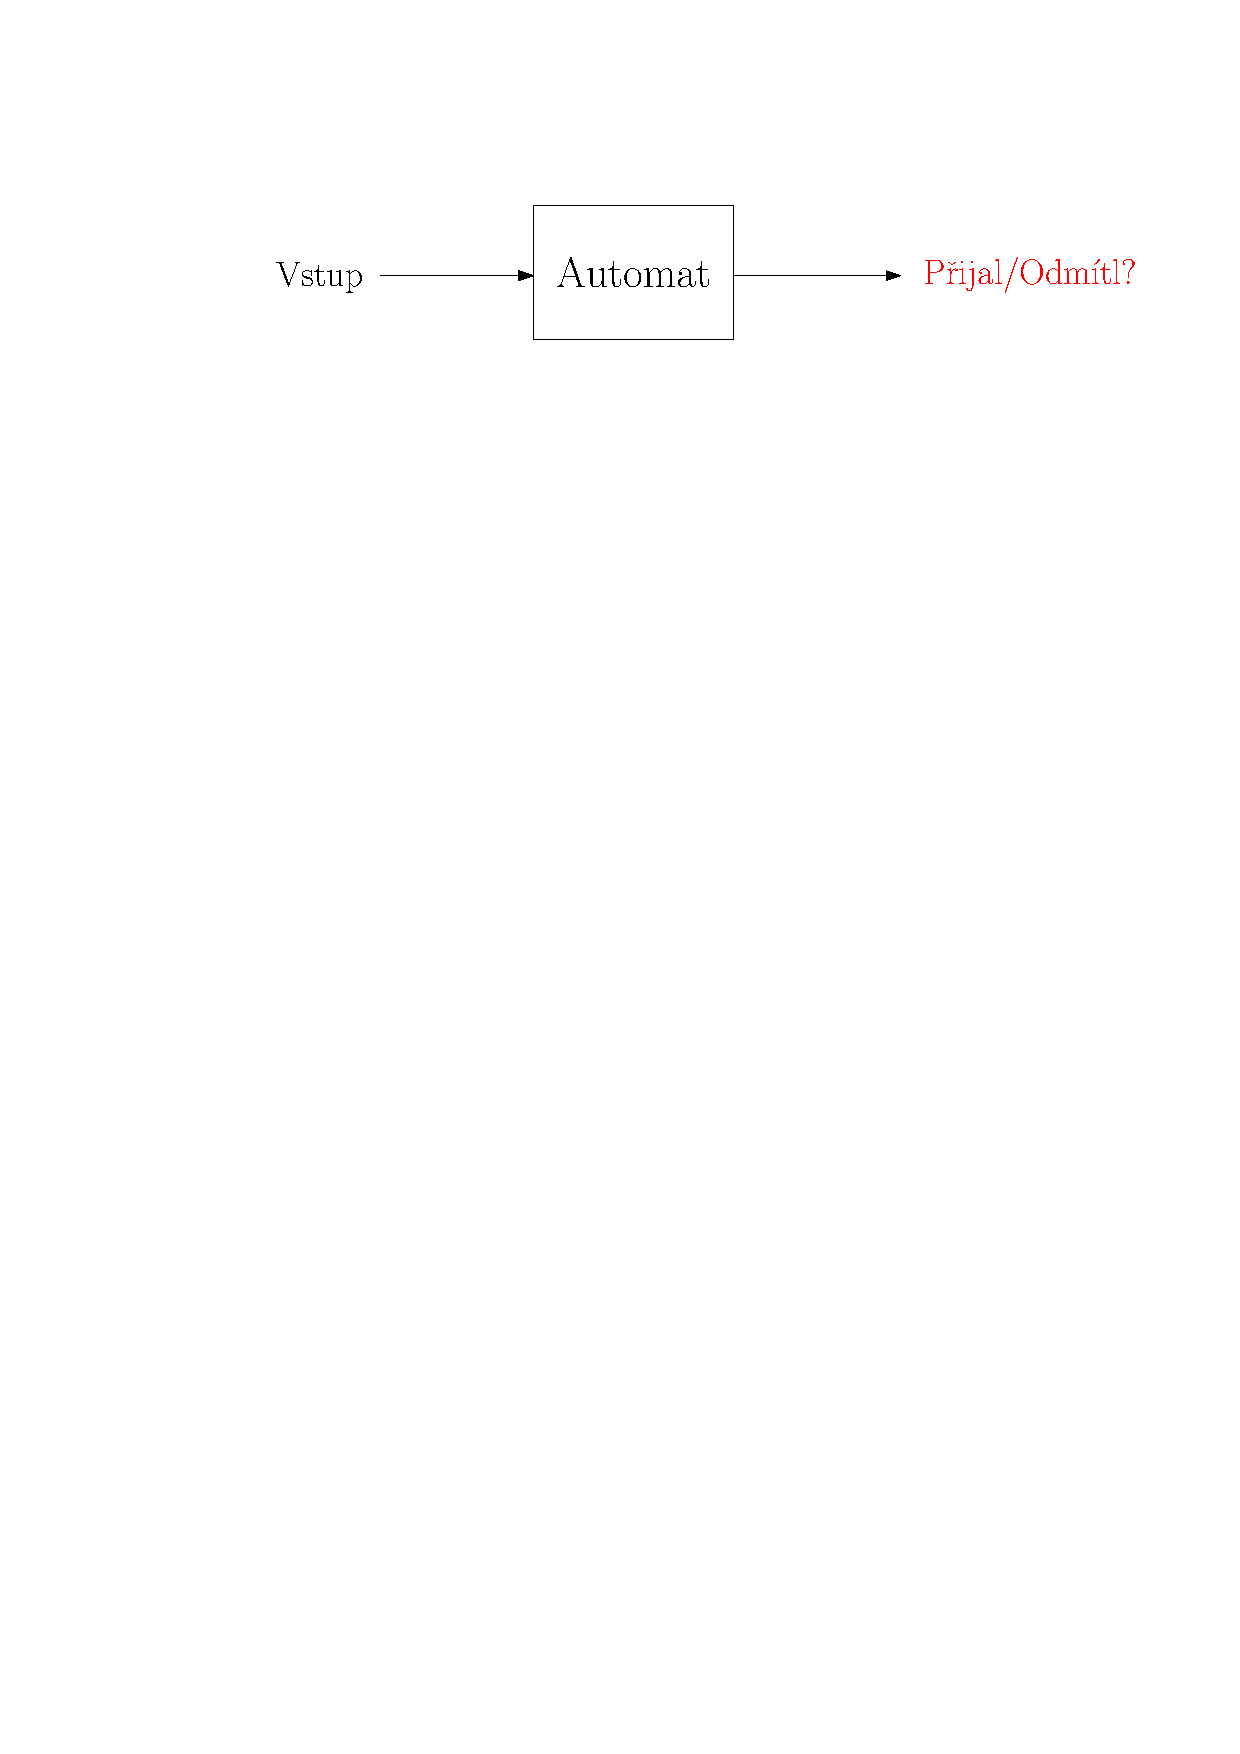
\includegraphics[scale=.7]{03-automaty/images/ch03_konecny-automat.pdf}
    \caption{Zjednodušené schéma konečného automatu.}
    \label{fig:konecny-automat}
\end{figure}